\documentclass{article}
\usepackage[utf8]{inputenc}
\usepackage{subfig}
\usepackage{amsmath}

\usepackage{graphicx}
\usepackage[legalpaper, landscape, margin=0.5cm]{geometry}

\thispagestyle{empty}
% \renewcommand{\thesubfigure}{\roman{subfigure}}
\begin{document}

\begin{figure}[h]
        \centering
        \subfloat[profile]{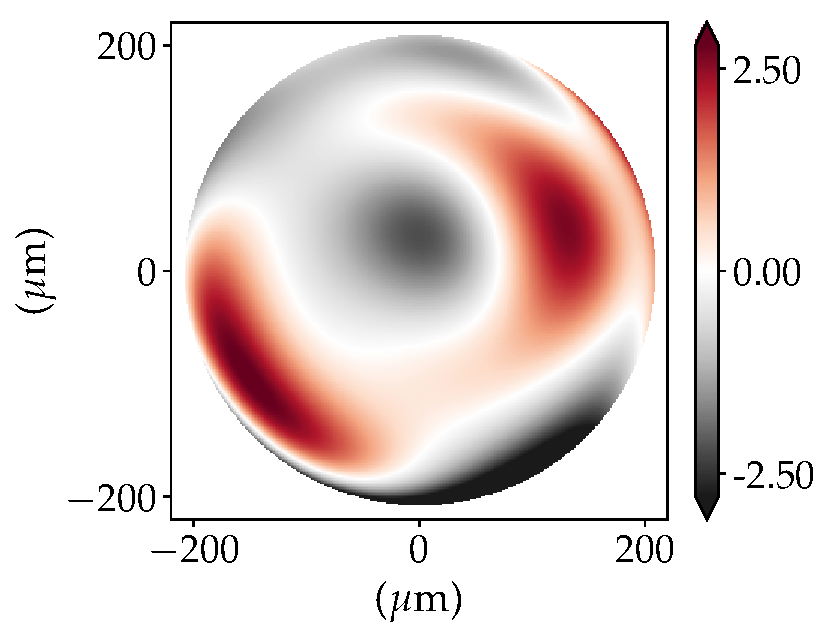
\includegraphics[height=3.4cm]{figures/ch04/figure_errors_LF_workflow_a_FC_Be.pdf}}\hspace{0.1cm}        
        \subfloat[PSF]{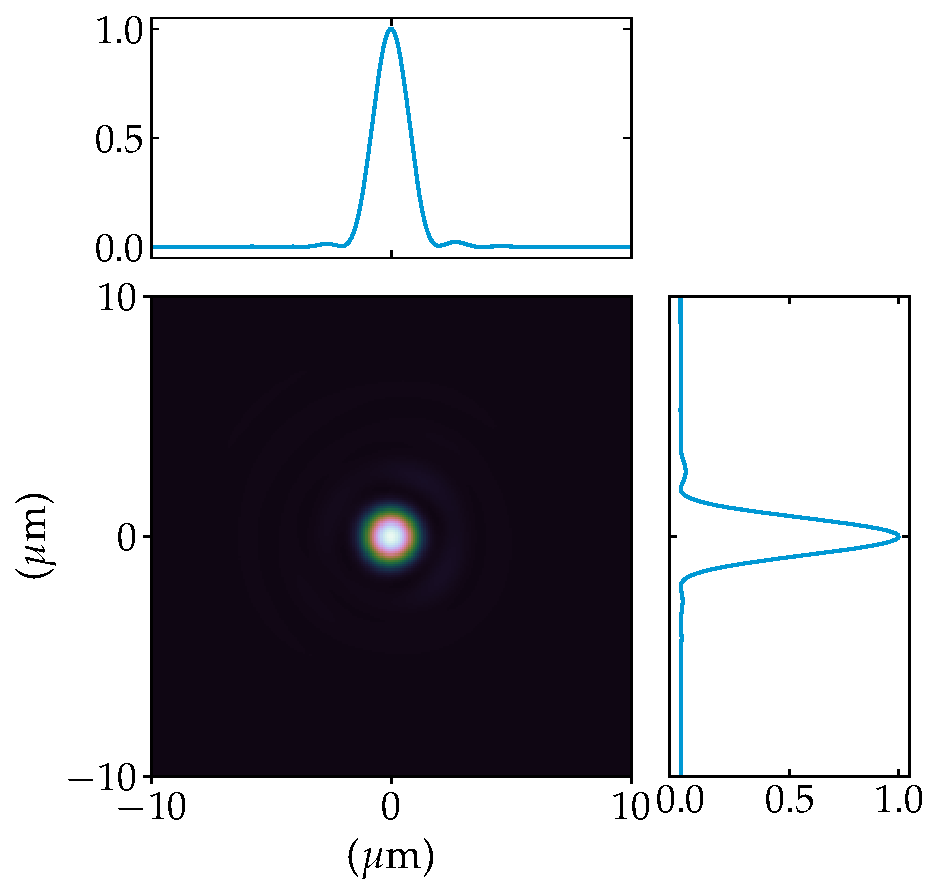
\includegraphics[height=5cm]{figures/ch04/cst_CRL_Be_Zernike_intensity_intensity_2D.pdf}}\hspace{0.1cm}
        \subfloat[vertical caustics]{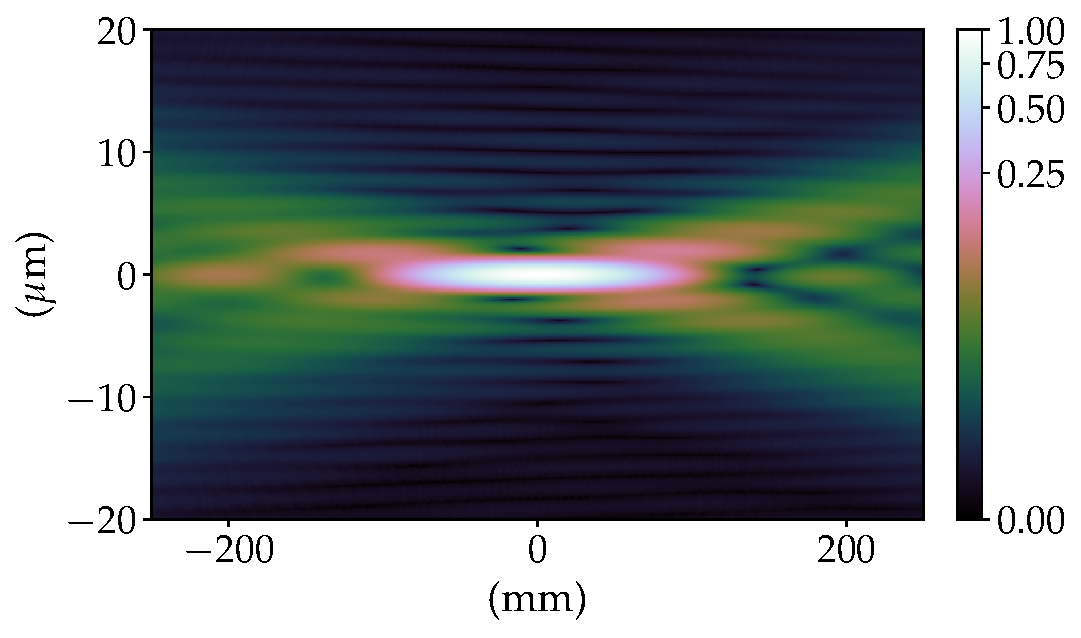
\includegraphics[height=3.5cm]{figures/ch04/cst_CRL_Be_metrology_intensity_cstc_Y_cstc_2D.pdf}}\\\caption*{Simulations using the Zernike circle polynomials}
        \subfloat[profile]{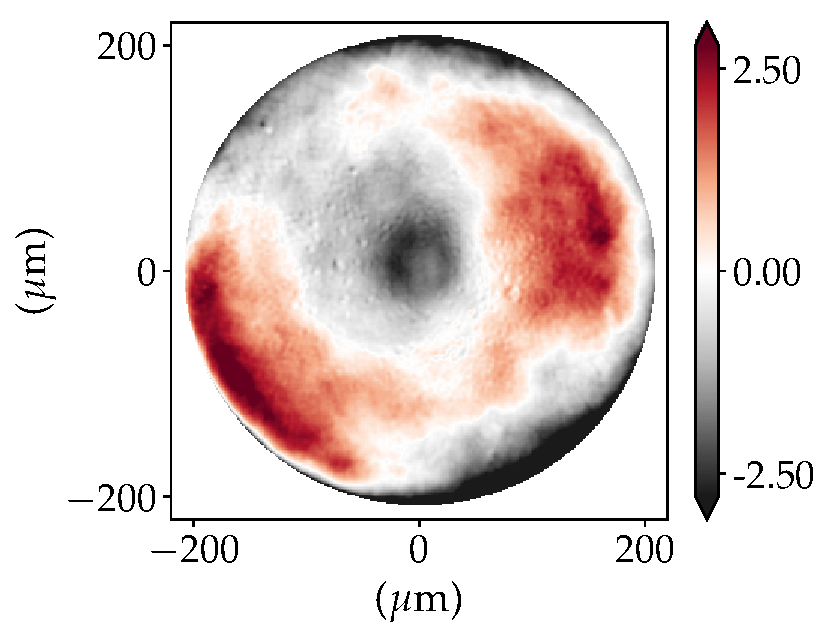
\includegraphics[height=3.4cm]{figures/ch04/figure_errors_FF_workflow_a_FC_Be.pdf}}\hspace{0.1cm}        
        \subfloat[PSF]{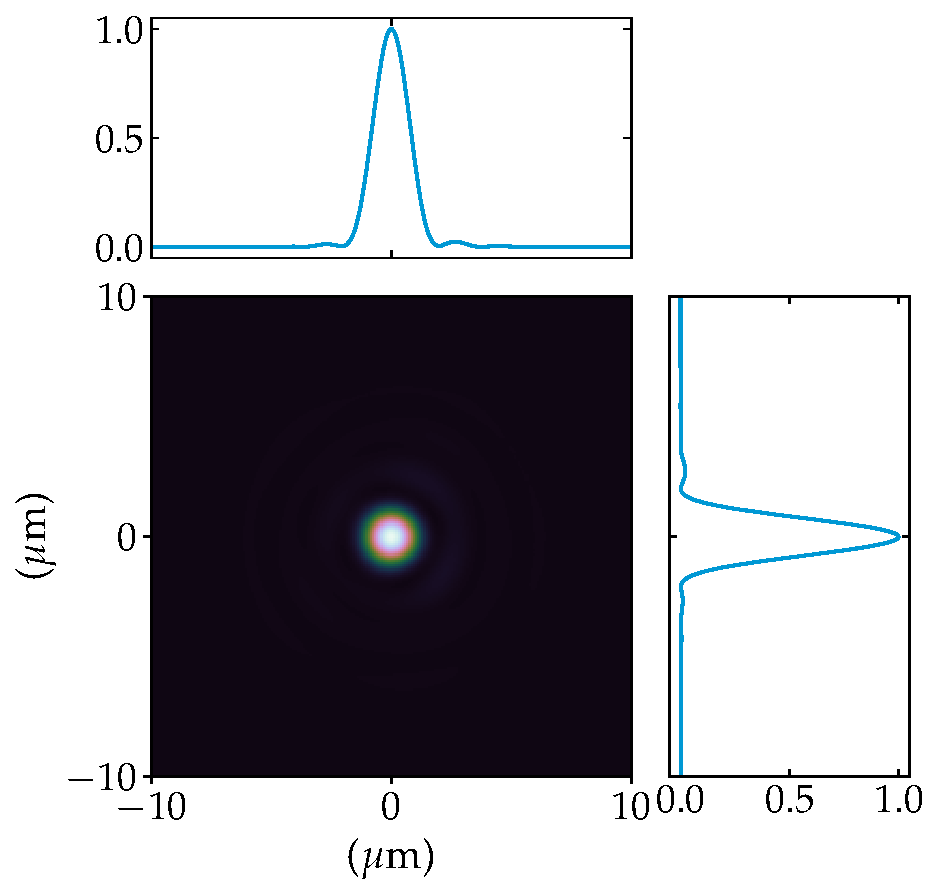
\includegraphics[height=5cm]{figures/ch04/cst_CRL_Be_metrology_intensity_intensity_2D.pdf}}\hspace{0.1cm}
        \subfloat[vertical caustics]{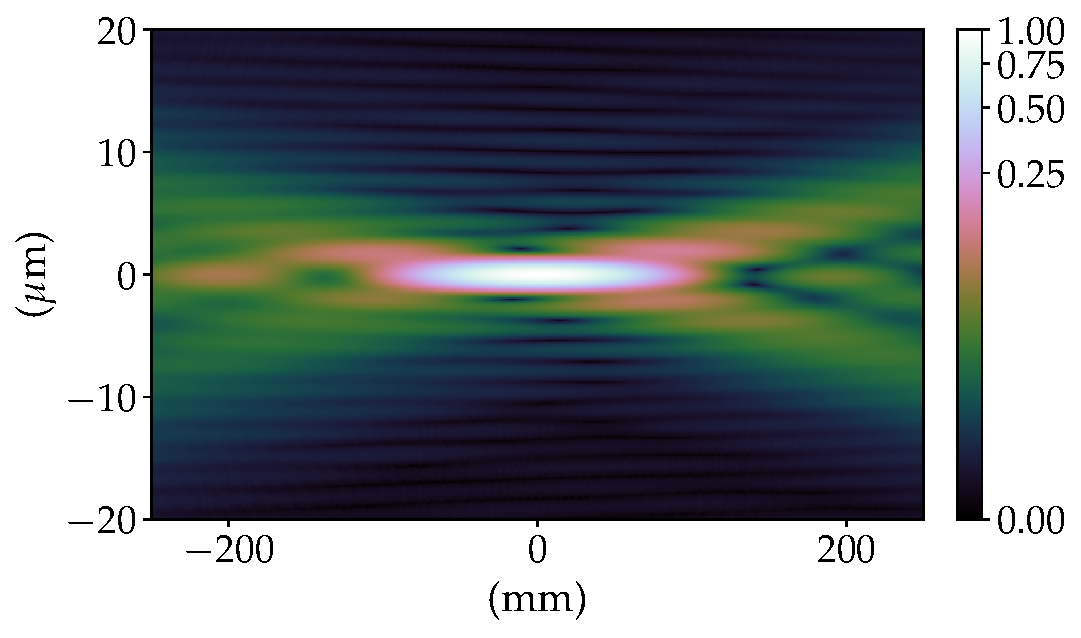
\includegraphics[height=3.5cm]{figures/ch04/cst_CRL_Be_metrology_intensity_cstc_Y_cstc_2D.pdf}}\\\caption*{Simulations using the metrology data}
\end{figure}
\end{document}

